% Number 821
% CAPMG Units 
% Rocket launch, freefall afterwards - difficult graphical
% JG

% Watermark
\AddToShipoutPicture*{\BackgroundPic}

\addtocounter {ProbNum} {1}

%\begin{floatingfigure}[r]{.44\textwidth}
%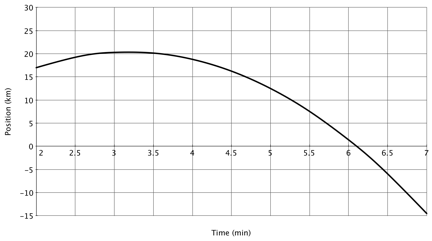
\includegraphics[scale=.5]{/Users/jgates/desktop/latex/pics/xgraph2}
%\end{floatingfigure}
 
{\bf \Large{\arabic{ProbNum}}} A rocket blasts off, traveling with an acceleration of ${4~\tfrac{m}{s^2}}$ upward.  When it is 2000 meters above the ground, its engine shuts off. \bigskip

How much time was required for the rocket to reach the 2000 meter altitude, and how fast was it moving at that moment? Use graphical methods.\paragraph{}
\noindent

%\begin{center}
%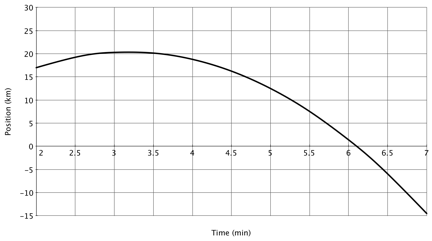
\includegraphics[scale=1]{/Users/jgates/desktop/latex/pics/xgraph2}
%\end{center}

\vfill
\newpage